\scanpage{11}
geometricqlly irr\tikz[baseline=(s.base)]{\node[inner sep=0pt](s){e};\draw[line width=1pt] ([xshift=.2pt,yshift=-.5pt]s.north)--++(0,3pt);}ducible, i.e. $\underline{D}$ is constant, and assume $B$ geometrically regular over $k$. This second condition implies that $X\handwritten{\widehat{\mathord{\tikz[baseline=(s.base)]{\node[inner sep=0pt](s){$\mathrm{x}$};\draw[line width=.5pt] ([xshift=.5pt,yshift=1.3pt]s.center) ellipse[x radius=3pt,y radius=4.5pt];}}}}_k B$ is regular, and denoting by $U\handwritten{\widehat{\mathord{\tikz[baseline=(s.base)]{\node[inner sep=0pt](s){$\mathrm{x}$};\draw[line width=.5pt] ([xshift=.5pt,yshift=1.3pt]s.center) ellipse[x radius=3pt,y radius=4.5pt];}}}}_k B$ the inverse image of $U$ in this scheme, \deleted{the}\tikz[baseline=(s.base)]{\node[inner sep=0pt](s){x};}\deleted{first condition}\tikz[baseline=(s.base)]{\node[inner sep=0pt](s){x};}\deleted{\unsure{t|i}} this tog\rlap{t}e\rlap{e}ther with the first condition implies that \deleted{the} \tikz[baseline=(s.base)]{\node[inner sep=0pt](s){\deleted{\unsure{right}}};\node[anchor=south,inner sep=0pt] at ([yshift=3pt]s.north){\inserted{\deleted{left}}};}\deleted{ hand side of (20)}\tikz[baseline=(s.base)]{\node[inner sep=0pt](s){is};\node[anchor=south west,inner sep=1pt](a) at ([xshift=-4em,yshift=7pt]s.north west){\inserted{\handwritten{$\operatorname{Pic}(X\widehat{\otimes}_k B)/\underline{D}(B)$}}};\draw ([xshift=-3pt,yshift=-2pt]s.south west) to[out=90,in=180] ([xshift=0pt,yshift=-2pt]a.south west)--([xshift=0pt,yshift=-2pt]a.south east) to[out=0,in=-90] ([xshift=3pt,yshift=3pt]a.south east);} isomorphic to $\operatorname{Pic}(U\handwritten{\widehat{\mathord{\tikz[baseline=(s.base)]{\node[inner sep=0pt](s){$\mathrm{x}$};\draw[line width=.5pt] ([xshift=.5pt,yshift=1.3pt]s.center) ellipse[x radius=3pt,y radius=4.5pt];}}}}_k B)$. This shows that o n the sub-category of arguments $B$ which are \deleted{g\unsure{e}} noetherian and geometrically regular, $Q$ is the étale sheaf associated to the presheaf
\[
\begin{aligned}
(21)\qquad\qquad & B\handwritten{\longmapsto}\operatorname{Pic}(U\handwritten{\widehat{\mathord{\tikz[baseline=(s.base)]{\node[inner sep=0pt](s){$\mathrm{x}$};\draw[line width=.5pt] ([xshift=.5pt,yshift=1.3pt]s.center) ellipse[x radius=3pt,y radius=4.5pt];}}}}_k B)\handwritten{/\operatorname{Pic}(B)}\deleted{\unsure{(}}\handwritten{(\hookrightarrow}Q(B))\ .
\end{aligned}
\]
The obstruction for an element of $Q(B)$ to belong to $\operatorname{Pic}(U\handwritten{\widehat{\mathord{\tikz[baseline=(s.base)]{\node[inner sep=0pt](s){$\mathrm{x}$};\draw[line width=.5pt] ([xshift=.5pt,yshift=1.3pt]s.center) ellipse[x radius=3pt,y radius=4.5pt];}}}}_k B)$ \tikz[baseline=(s.base)]{\node[inner sep=0pt](s){is};\node[anchor=south west,inner sep=1pt](a) at ([xshift=-.5em,yshift=7pt]s.north west){\inserted{\handwritten{$/\operatorname{Pic}(B)$}}};\draw ([xshift=-3pt,yshift=-2pt]s.south west) to[out=90,in=180] ([xshift=0pt,yshift=-2pt]a.south west)--([xshift=0pt,yshift=-2pt]a.south east) to[out=0,in=-90] ([xshift=3pt,yshift=3pt]a.south east);} in the Brauer group $\operatorname{Br}(B)$. Thus, unde\rlap{e}r very stringent conditions on $B$ at least (being geometrically regular) we get a description of $Q(B)$ in terms of actual local Picard groups. I should have sta\rlap{e}ted that $U\handwritten{\widehat{\mathord{\tikz[baseline=(s.base)]{\node[inner sep=0pt](s){$\mathrm{x}$};\draw[line width=.5pt] ([xshift=.5pt,yshift=1.3pt]s.center) ellipse[x radius=3pt,y radius=4.5pt];}}}}_k B$ can also be interpreted as the inverse image of $U$ in the scheme $\unsure{\mathbb{S}|S}\mathrm{pec}(A\handwritten{\widehat{\mathord{\tikz[baseline=(s.base)]{\node[inner sep=0pt](s){$\mathrm{x}$};\draw[line width=.5pt] ([xshift=.5pt,yshift=1.3pt]s.center) ellipse[x radius=3pt,y radius=4.5pt];}}}}_k B)$, and thus makes a sense independently of the choice of a particular resolution.

One may wish to construct a local Picard scheme \deleted{without} also in case $A$ is not equi-caracteristic, which implies that $\mathrm{car}.k\handwritten{>}0$. It seems likely that this can be done if $k$ is perfect. The key-point here \deleted{seems} \deleted{to} is the construction of schemes $P_n$, which leads us to the foll\rlap{w}o\rlap{o}wing

\uline{\rlap{B}Problem}\quad Let $A$ be a local Artin ring with perfect residue field $k$ of car. $p\handwritten{>}0$, $X$ a proper scheme over $A$. Give a ``natural'' constructio\unsure{n} of a group scheme locally of finite type $P$ over $k$, together with an imbedding
\margin{\figure{\handwritten{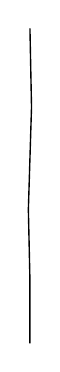
\begin{tikzpicture}\draw[line width=.5pt] (0,0)--(.02,-1)--(-.02,-2.3)--(0,-3.2)--(0,-4);\end{tikzpicture}}}}
\[
\begin{aligned}
(22)\qquad\qquad & \operatorname{Pic}(X)\handwritten{\hookrightarrow}P(k)\ ,
\end{aligned}
\]
the obstruction for an element of $P(k)$ to beling to $\operatorname{Pic}(X)$\handwritten{(}being in $\operatorname{Br}\ H^o(X,\underline{O}_X)$, and hence\handwritten{)}vanishing if $k$ is algebraically close\rlap{e}d.
% archive sheet number: 10
